% Papers due Nov. 21
% TODO: Put a reference for Figure 2
% TODO: Near line 200, is the wave data used for dot_z?
%
% Carlos comment on the necessity of RM3 discussion has been addressed by merging sections II and III.
% Added a bit to the end of section III to stress that PTO-Sim will aim for all PCCs

\documentclass[conference]{IEEEtran}
\usepackage{graphicx}
\usepackage{epstopdf}
\usepackage{dblfloatfix}
\usepackage{cite}

%\usepackage[latin9]{inputenc}
%\usepackage{color}
%\usepackage{array}
%\usepackage{float}
%\usepackage{multirow}
%\PassOptionsToPackage{normalem}{ulem}
%\usepackage{ulem}
%\makeatletter
%\newcommand{\noun}[1]{\textsc{#1}}
%\providecommand{\tabularnewline}{\\}
% correct bad hyphenation here

\hyphenation{op-tical net-works semi-conduc-tor}
\makeatother


\begin{document}

\title{
    PTO-Sim: Development of a Power Take Off Modeling Tool for Ocean Wave Energy Conversion
    }


\author{
    \IEEEauthorblockN{
        Ratanak So\textsuperscript{1}, \textit{Student Member, IEEE},
        Sean Casey\textsuperscript{2},
        Sam Kanner\textsuperscript{3},
        Asher Simmons\textsuperscript{1}, \textit{Student Member, IEEE},\\
        Ted K. A. Brekken\textsuperscript{1}, \textit{Senior Member, IEEE}
     }\\
    \IEEEauthorblockA{
    \textsuperscript{1}Oregon State University} 
    \IEEEauthorblockA{
    \textsuperscript{2}Engergy Storage Systems, Inc.}
    \IEEEauthorblockA{
    \textsuperscript{3}University of California Berkeley}
%    \IEEEauthorblockA{
%        School of Electrical Engineering and Computer Science\\
%        Oregon State University\\
%        Corvallis, Oregon 97331\\
%        Email: brekken@eecs.oregonstate.edu} 
        }
\maketitle


\begin{abstract}
Sandia National Laboratories (SNL) and National Renewable Energy Laboratory (NREL) have collaborated to develop the open-source Wave Energy Converter (WEC) modeling tool WEC-Sim, capable of running on a standard personal computer. Its main function is to simulate WECs of arbitrary geometry subject to operational waves; both regular and irregular waves. However, WEC-Sim Version 1.0 models a power take-off (PTO) as a simple linear damper. A collaborative effort between SNL and the Energy Systems group at Oregon State University (OSU) has resulted in the development of PTO-Sim, an additional WEC-Sim library for accurately modeling a WEC PTO system such as hydraulic or direct-drive. This development of PTO-Sim makes WEC-Sim a wave-to-wire model by adding functionality that extends WEC-Sim capabilities. The WEC PTO system is easily created with drag and drop PTO-Sim library blocks to build a model that can estimate absorbed and electrical power.   
\end{abstract}


\begin{IEEEkeywords}
WEC-Sim, PTO-Sim, hydraulic, absorbed power, mechanical power, electrical power. 
\end{IEEEkeywords}

\section{WEC-Sim Overview}

WEC-Sim is an open-source WEC simulation tool that is developed in MATLAB/Simulink using the multi-body dynamics solver SimMechanics \cite{wecsim}. WEC-Sim relies on Boundary Element Method (BEM) codes, such as WAMIT, to obtain hydrodynamic coefficients such as added mass, radiation damping, and wave excitation. SNL and NREL have completed the code verification by comparing results against commercially available codes \cite{ruehl2014preliminary}\cite{ruehl2014development}. WEC-Sim Version 1.0 models WEC devices as a combination of rigid bodies, joints, linear PTOs, and mooring systems \cite{yu2014design}\cite{lawson2014implementing}. 

\section{WEC-Sim Motivation}
The main goal of developing WEC-Sim is to promote and support the wave energy industry. Since WEC-Sim is an open-source WEC code and uses a time domain modeling method which is capable of running on a standard personal computer, it is very convenient to operate. Users can choose from a variety of different WEC-Sim library blocks to model different WECs.  As an illustrative example, WEC-Sim modeling of Reference Model 3 (RM3) is shown in Fig. 1  \cite{wecsim}\cite{ruehl2014preliminary}.  Reference Model 3 (RM3) is the result of the DOE-funded Reference Model Project and has been adopted by many wave energy developers in the WEC industry due to its relatively simple operating principles \cite{sandia}. RM3 is a simple two-body point absorber, consisting of a float and a reaction plate. The float is connected to the spar/plate through a translational joint with a defined linear damping coefficient that simulates the PTO system, and the spar/plate is connected to the seabed through a 6 degrees of freedom (DOF) floating connection.

\begin{figure}[t]
    \centering
    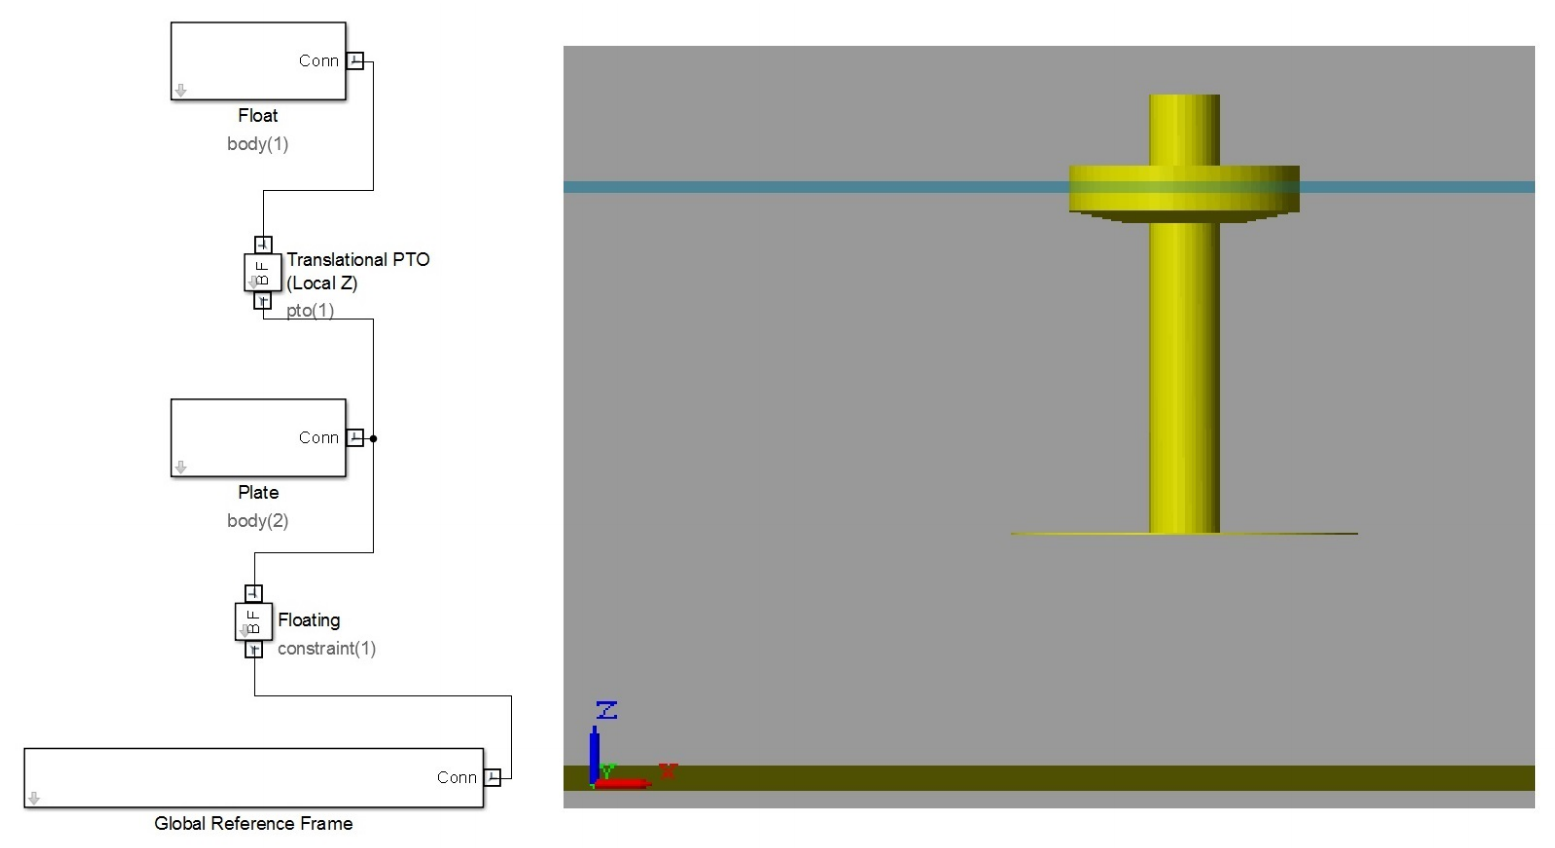
\includegraphics[width=1\columnwidth]{Images/RM3}
    \caption{RM3 model in WEC-Sim (left) and with the animation (right) [1].}
    %\label{fig-freq-comparison}
    \end{figure}

\section{Power Conversion Paths}

% TB: Double column floats get put after the page they are instantiated in, so I put it at the beginning to get it to appear on the next page where it fit better
\begin{figure*}[t] 
    \centering
    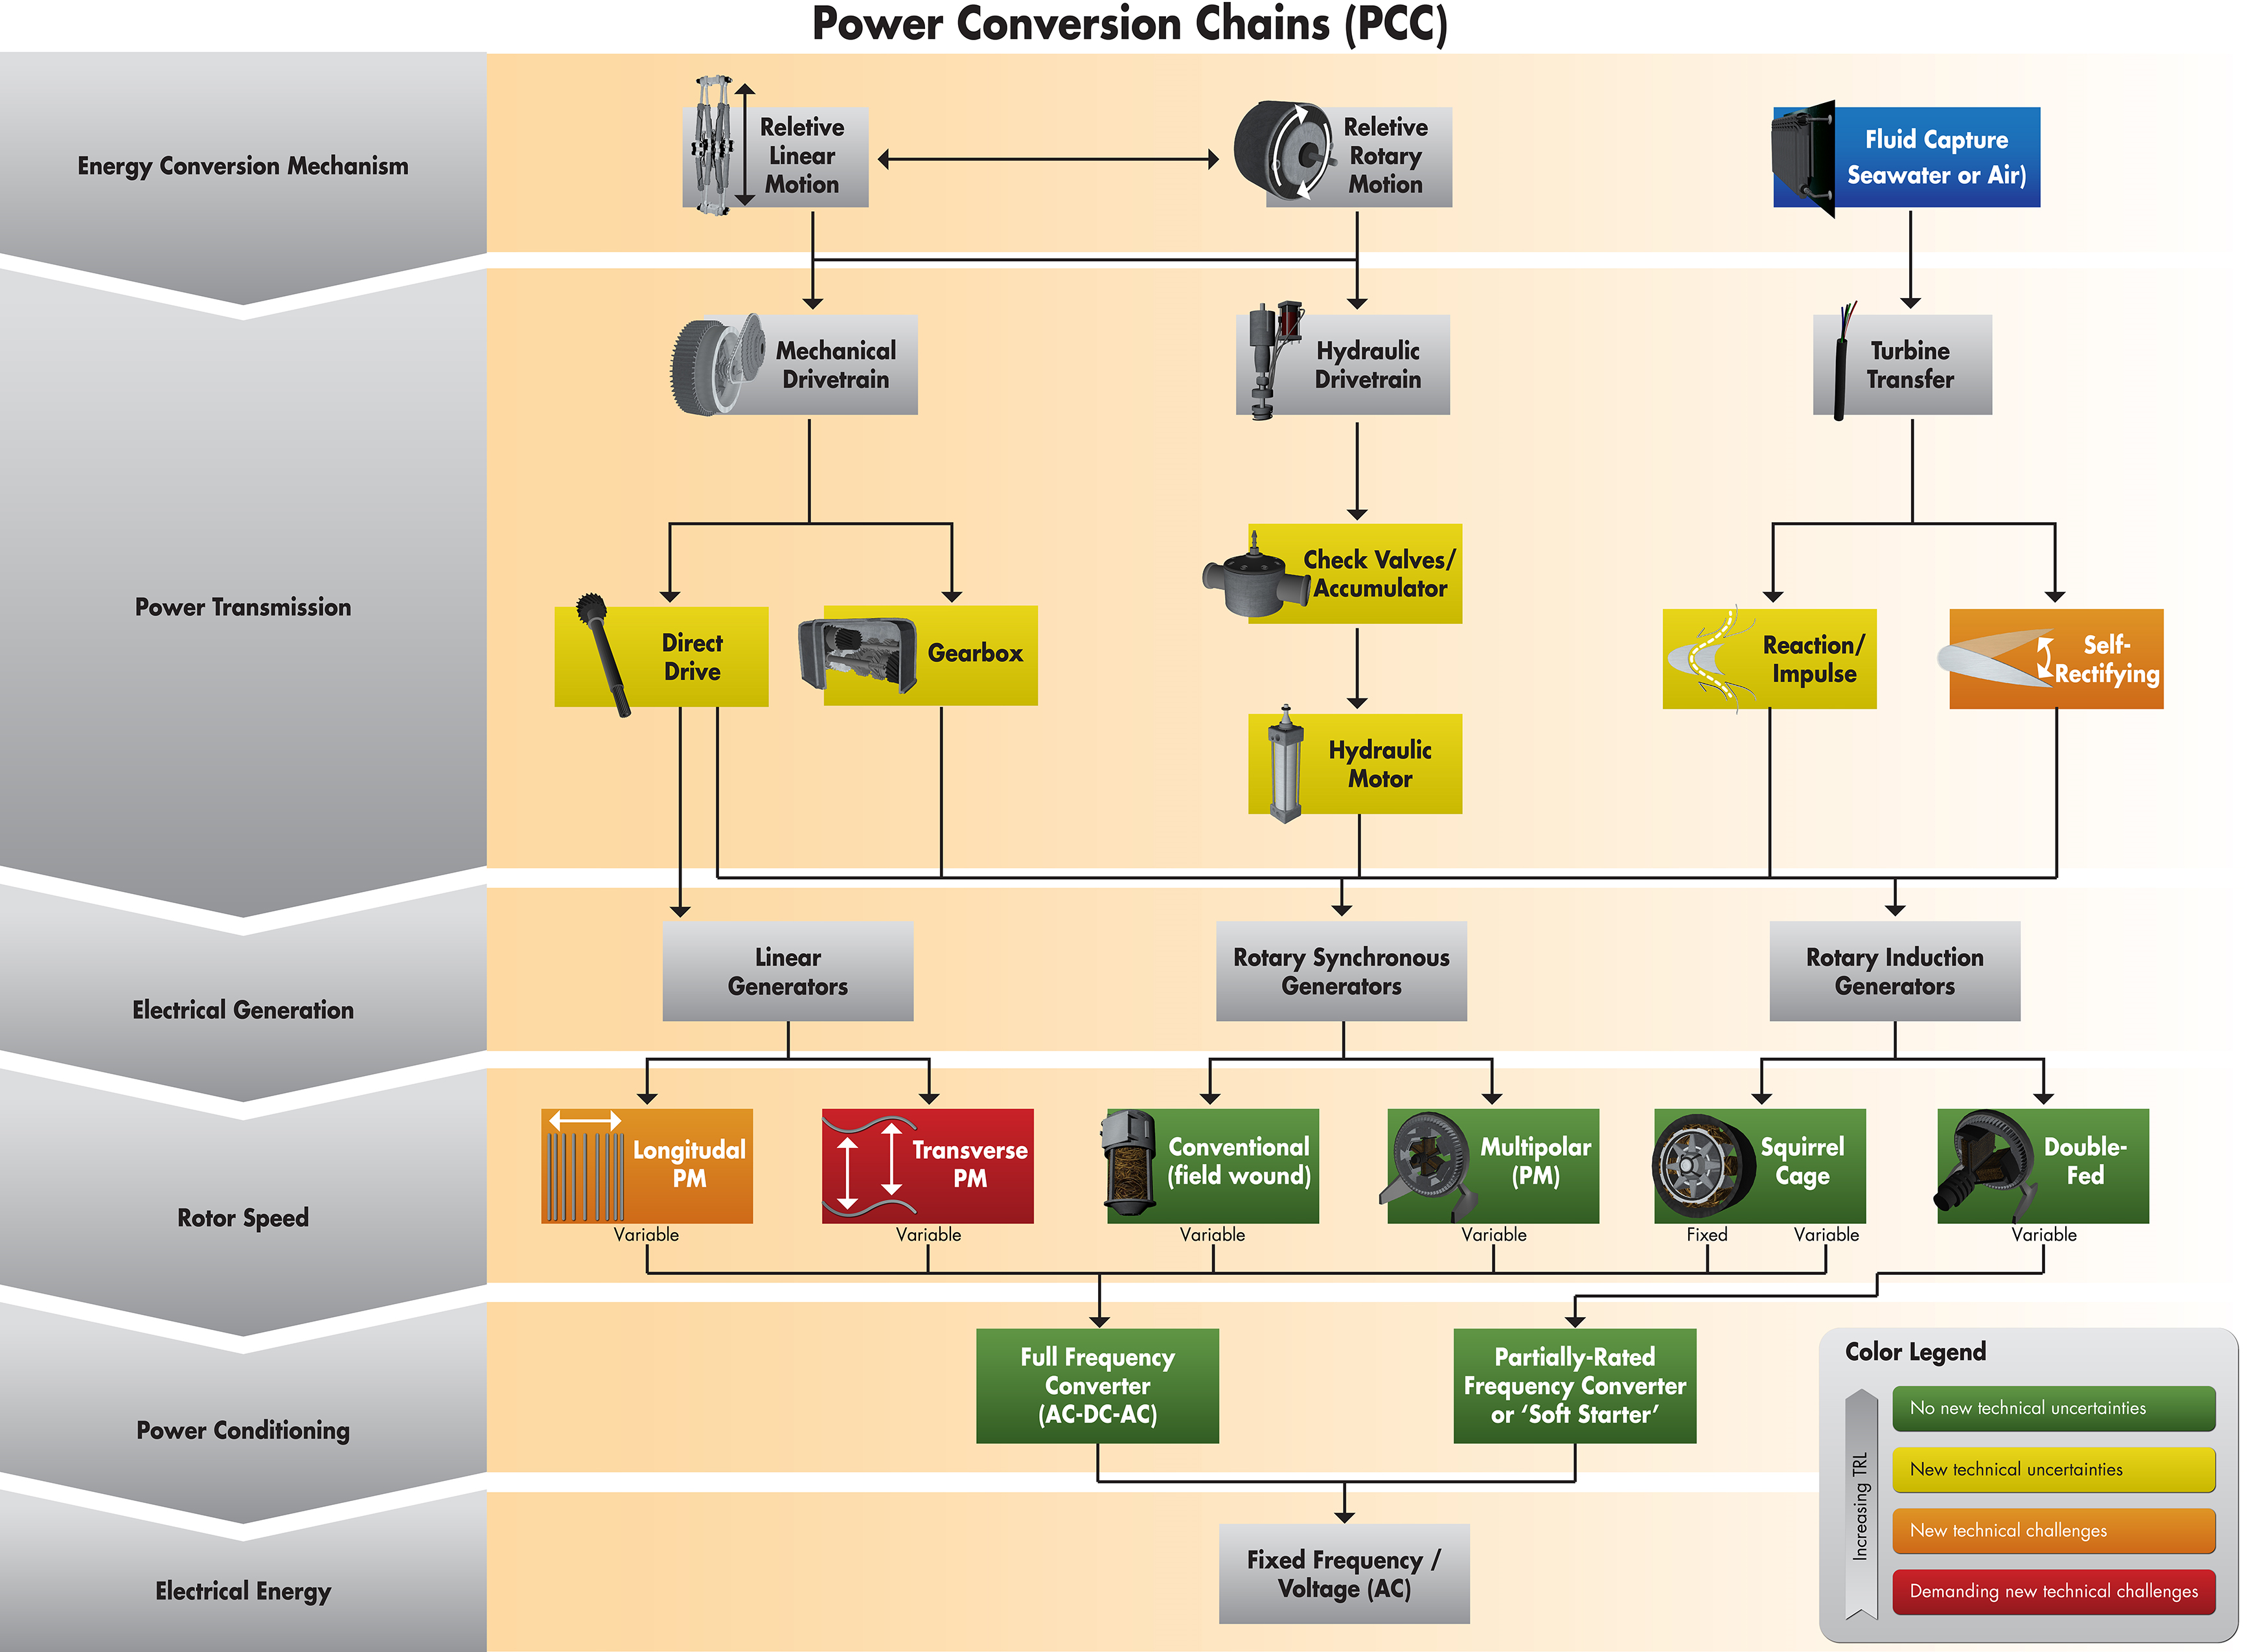
\includegraphics[width=1.95\columnwidth]{Images/PCC}
    \caption{Power conversion chain from mechanical energy to electrical connection to grid. Lower TRLs are novel concepts and higher TRLs are more proven technology.}
    %\label{fig-freq-comparison}
    \end{figure*}

\begin{figure}[t]
    \centering
    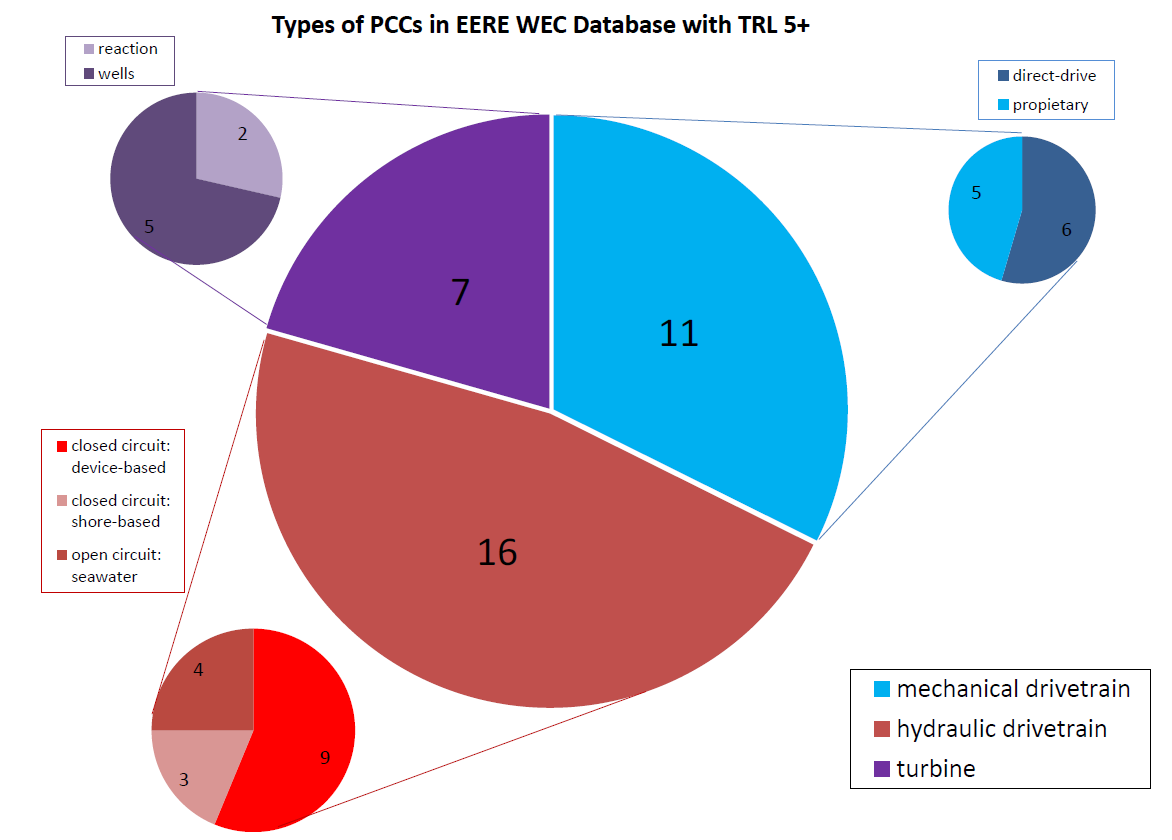
\includegraphics[width=1\columnwidth]{Images/TRL}
    \caption{Breakdown of PCC types currently used by companies with TRL equal to or greater than 5.}
    %\label{fig-freq-comparison}
    \end{figure}

Nearly all WECs convert energy from the wave into either relative linear motion, relative rotary motion, or fluid capture. The power conversion chain (PCC) converts this mechanical power into electrical power.  There are several methods used to convert the mechanical power to electrical power. As shown in Fig. 2, the different PCCs are usually associated with different categories of mechanical motion. On the left side of the figure is a conceptual energy conversion flow. On the right side, black arrows indicate possible power flow paths. The ``Color Legend" represents a grouping of technology while colors refer to technological readiness categorization \cite{reed2010accelerating}\cite{ruehl2012wave}. The technological readiness categorization in Fig. 2 is based on the work in the DNV Recommended Practices, found in \cite{veritas2001recommended}, which takes into consideration the degree of the novelty of the technology as well as the application area. 

According to the EERE WEC database as shown in Fig. 3, there are 34 PCCs that are at or beyond technology readiness level (TRL) 5. Of these 34, 16 use a hydraulic drive train \cite{eere}. And, of the remaining 18 devices, 7 do not indicate a generator technology. These statistics indicated that the PTO-Sim library development should begin with the elements of the hydraulic drive train.  The end-goal for PTO-Sim will be to model all of the Power Conversion Chain options shown in Fig. 2.


    
\section{PTO-Sim Motivation}
Due to the popularity of hydraulic drivetrains among current WEC developers, a hydraulic module has been included in PTO-Sim. A hydraulic PTO modeled in native MATLAB/Simulink will replace a simple linear damper PTO model that is used by the current release of WEC-Sim (Version 1.0).

SNL and the Energy Systems group at Oregon State University (OSU) have collaborated in the development of PTO-Sim, the WEC-Sim sub-system responsible for accurately modeling a WEC PTO system. This development of PTO-Sim makes WEC-Sim a wave-to-wire model by adding functionality that natively extends WEC-Sim capabilities. The WEC PTO system is easily created with drag and drop PTO-Sim library blocks. 

\section{Hydraulic PTO}

A hydraulic PTO represents by the schematic in Fig. 4 is a system that the piston is assumed to be directly coupled to the buoy. The system begins with  a double acting hydraulic piston pump, labelled ``P", which converts the linear motion of the heaving buoy into a pressurized fluid flow. The bi-directional fluid flow from terminals ``A" and ``B" of the pump is passed through rectifying check valves, which change the bidirectional flow into a uni-directional flow. The valves with their assigned numbers ``1" through ``4" indicate the different flow paths. The uni-directional flow is delivered to the high pressure side of the system. The high pressure accumulator ``C" stores hydraulic energy and smoothes the fluid flow across the motor. A variable displacement motor ``M" translates the hydraulic fluid power into rotational energy which is used to spin a generator ``G". The fluid then enters the low pressure side where accumulator ``D" provides a pressurized reservoir for the hydraulic fluid. The pump draws fluid from the reservoir as needed to complete the circuit \cite{casey2013modeling}.

\begin{figure}[t]
    \centering
    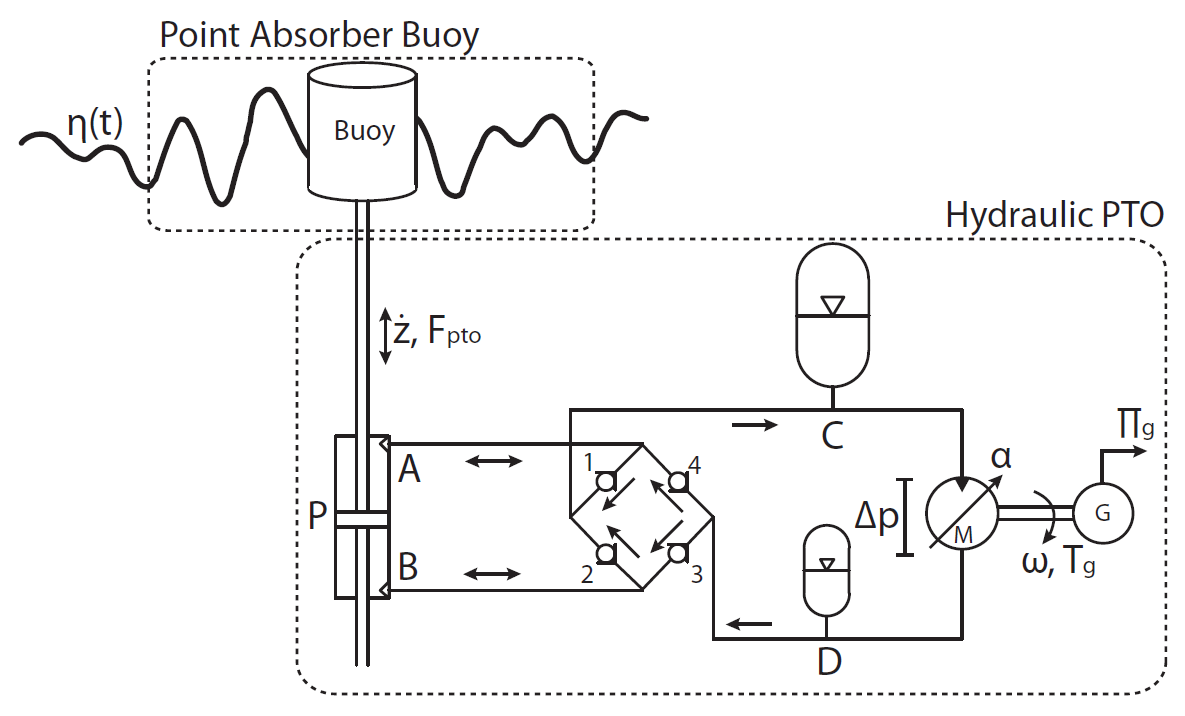
\includegraphics[width=1\columnwidth]{Images/HydraulicPTO}
    \caption{Schematic of the PTO-Sim hydraulic model. The arrow indicate the direction of flow.}
    %\label{fig-freq-comparison}
    \end{figure}



The hydraulic PTO model is described by equations (1) through (9). The pressure in line ``A" and ``B" is expressed using the continuity equation for a compressible fluid \cite{merritthydraulic}, as 

\begin{equation}
\dot{p}_A=\frac{\beta_e}{V_o-A_pz}(A_p\dot{z}-\dot{V_1}+\dot{V_4}) 
\end{equation}

\begin{equation}
\dot{p}_B=\frac{\beta_e}{V_o+A_pz}(-A_p\dot{z}-\dot{V_2}+\dot{V_3}) 
\end{equation}
%
where $\beta_e$ is the effective bulk modulus of the hydraulic fluid, $V_o$ is the initial volume of the cylinder, $A_p$ is the piston area, and $\dot{V}_1$ through $\dot{V}_4$ are the volumetric flows through each check valve with a corresponding numeric label in Fig. 4. The piston is assumed to be directly coupled to the buoy. Therefore, the velocity of piston, $\dot{z}$, is the same as the buoy. However, for the RM3 example, the spar does move (very small compared to the float) in the heave direction and so the relative velocity between the two bodies are used. 

The flow across each valve is modeled using the orifice equation as shown in (3), 

\begin{equation}
\dot{V}_i=C_dA_v \sqrt{\frac{2}{\rho}(p_j-p_k)\tanh(k_1(p_j-p_k))}  
\end{equation}
%
where $i=1,2,3,4$, $C_d$ is the discharge coefficient, $A_v$ is the area of the orifice described by (4), and $p_j$ and $p_k$  are the pressures on either side of the valve. The $tanh$ function was used because it was differentiable which is important for some control/optimization strategies as well as being easier for some ODE solvers to handle. The valve area is modeled as a variable area poppet valve,  

\begin{eqnarray}
A_v &=& A_{min}+\frac{A_{max}-A_{min}}{2}(1+\tanh(k_2(p_j-p_k)))\nonumber\\
&& +\frac{p_{max}+p_{min}}{2}
\end{eqnarray}
%
where $A_{max}$ and  $A_{min}$ are the maximum and minimum valve areas, $p_{min}$ is the cracking pressure, and $p_{max}$ is the pressure for which the valve is fully opened.  The $tanh$ function provides a smooth approximation to the step operation of the valve, where $k_2$ is chosen such that when the pressure difference is equal to the cracking pressure, the valve area is equal to $A_{min}$. The behavior of the valve can be seen in Fig. 5. 

\begin{figure}[t]
    \centering
    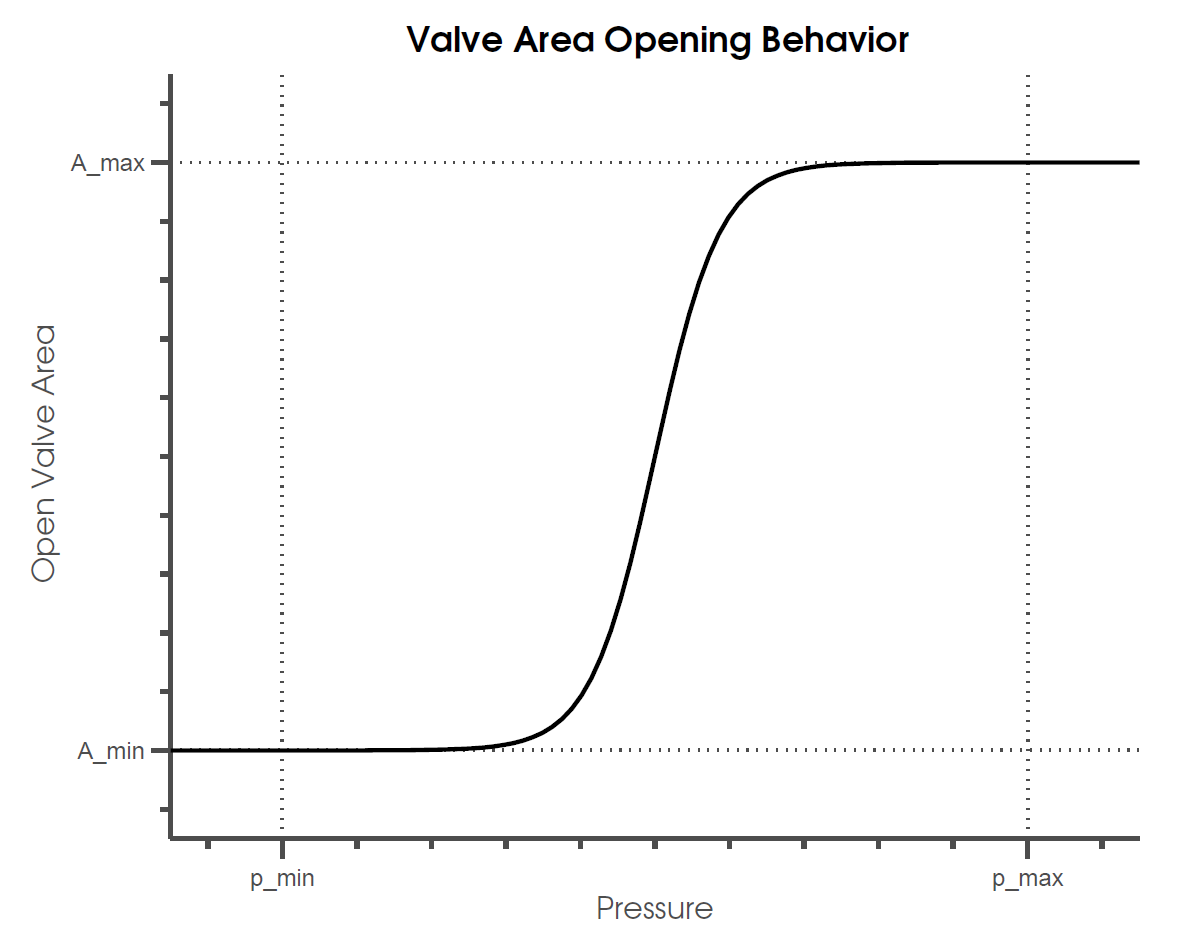
\includegraphics[width=1\columnwidth]{Images/ValveBehavior}
    \caption{Valve opening behavior as a function of pressure difference across the valve.}
    %\label{fig-freq-comparison}
    \end{figure}
    

\begin{figure*}[t]	
    \centering
    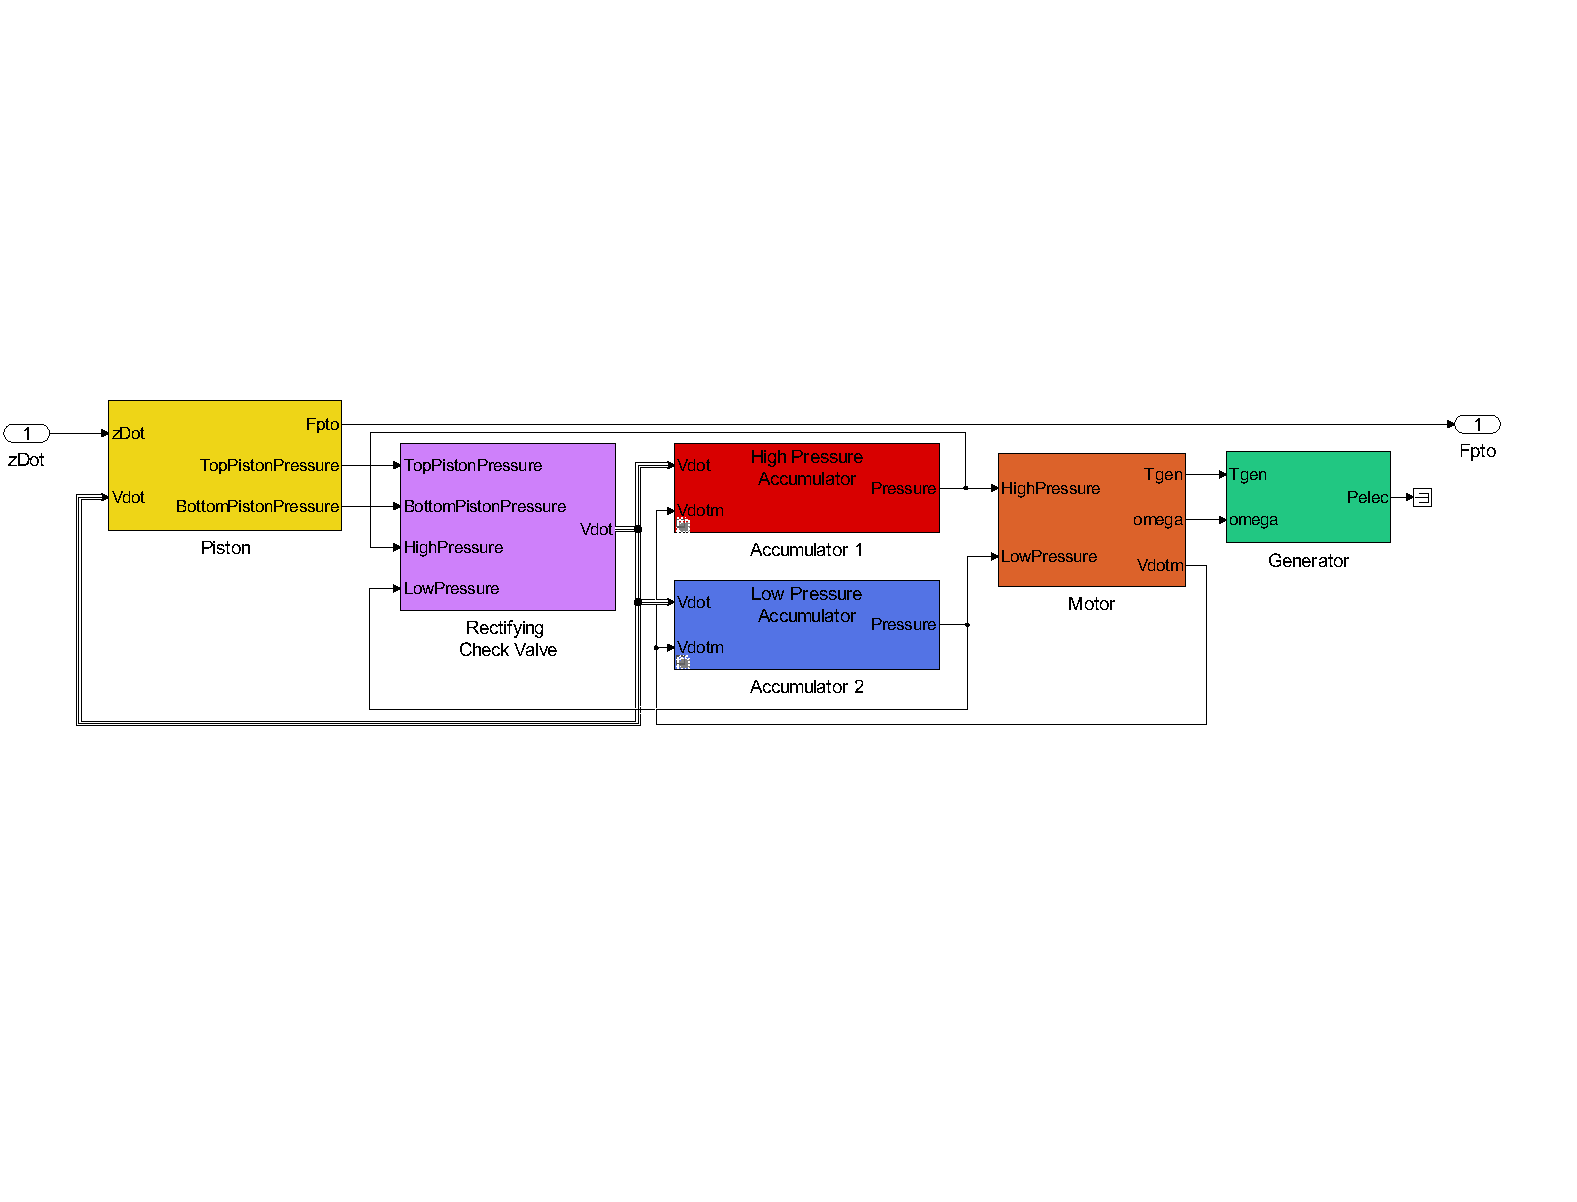
\includegraphics[width=2\columnwidth]{Images/ptomodel_color}  
    \caption{Simulink model of the hydraulic system.}
    \end{figure*}

The flow into accumulator ``C" and ``D" is described by (5) and (6) below
\begin{equation}
\dot{V}_C=-\alpha D \omega+\dot{V}_1+\dot{V}_2 
\end{equation}

\begin{equation}
\dot{V}_D=\alpha D \omega-\dot{V}_3-\dot{V}_4 
\end{equation}
%
where the flow across the motor is found using the swashplate angle ratio, $\alpha$, the nominal motor displacement, $D$, and the rotational speed of the generator, $\omega$. The swashplate angle ratio is a control input to vary the volumetric flow across the motor. The ratio represents the instantaneous motor displacement to the maximum motor displacement. For this hydraulic system the swashplate angle ratio is fixed for the simulated sea state. The pressure in each accumulator is dependent on the instantaneous volume of oil in the accumulator, related by

\begin{equation}
p_i=\frac{p_{i0}}{(1-\frac{V_i}{V_{i0}})^{1.4}}
\end{equation}
%
where $p_{i0}$ is the precharge pressure and $V_{i0}$ is the total volume of the accumulator. A torque balance on the hydraulic motor and generator drive leads to the state equation below

\begin{equation}
\dot{\omega}=\frac{1}{J_t}(\alpha D (p_C-p_D)-b_g \omega-b_f \omega)
\end{equation}
%
where $b_g$$\omega$ is the generator torque, $b_f$$\omega$ is the frictional torque, and $J_t$ is the total mass moment of inertia of the motor/generator drive train.  The frictional damping used was one that would give the generator a 95\% efficiency at a speed of 2400 rpm. 
The PTO force in (9) is determined by the pressure difference between sides A and B of the pump and the pressurized area of the piston, $A_p$.

\begin{equation}
F_{pto}=(p_A-p_B)A_p
\end{equation}

Fig. 6 is the hydraulic PTO model in Simulink. A user can drag and drop each module such as a Piston, Rectifying Check Valve, Accumulator, Motor, and Generator to build his or her own hydraulic PTO system. In this paper, PTO-Sim has not integrated with WEC-Sim yet. Therefore, the buoy velocity ``zDot" is assumed to be known.

\section{Simulation Results}
A hydraulic system was simulated in MATLAB/Simulink. Regular waves have been tested first in order to verify the model before moving on to irregular waves. 

An irregular wave with a significant wave height of 3 meters and a dominant period of 11 seconds is used.  The simulation results are shown in Figs. 7 through 10.  The average absorbed power is about 110 kW and the average electrical power is approximately 66 kW. Therefore, the efficiency is calculated to be 60~\%. 

\begin{figure}[t]
    \centering
    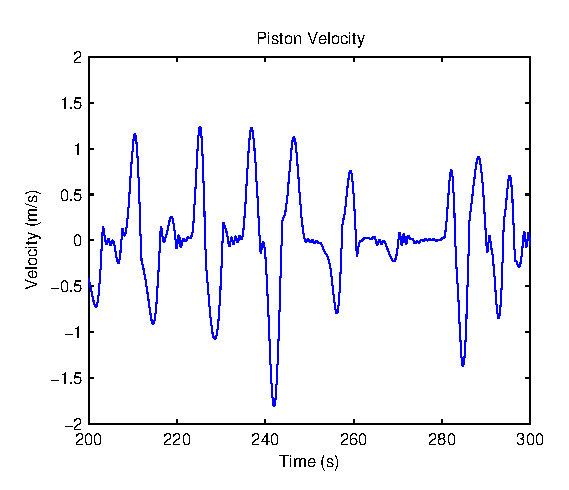
\includegraphics[width=1\columnwidth]{Images/zDot}
    \caption{Piston velocity for a wave of 3 meters with a dominant period of 11 seconds. The piston is assumed to be directly coupled to the buoy.}
    %\label{fig-freq-comparison}
    \end{figure}

Looking at the simulation time between 270 and 280 seconds, the buoy velocity is close to zero and there is not enough pressure on the piston side to open the check-valves. Figs. 8 and 9 show the system forcing and pressure when this phenomenon occurs. Since the fluid is modeled as compressible and the valves have trapped the fluid on the piston side, a spring-like effect occurs where the pressure on the piston side oscillates and decays until there is enough excitation force to open the valve. This hydraulic system therefore manifests an intrinsic latching control \cite{falnes2005ocean}.

\begin{figure}[t]
    \centering
    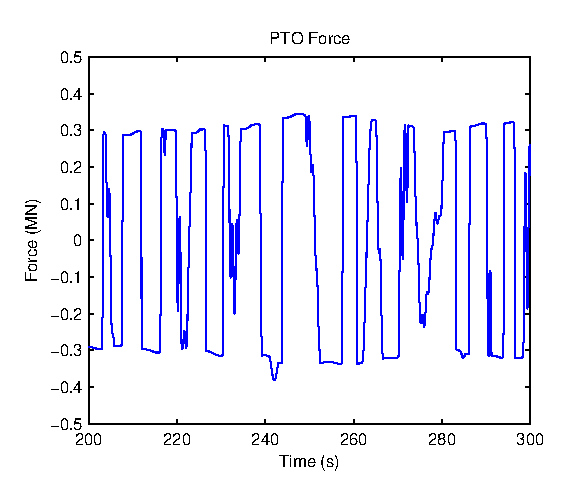
\includegraphics[width=1\columnwidth]{Images/ptoForce}
    \caption{Force applied by the PTO.}
    %\label{fig-freq-comparison}
    \end{figure}

\begin{figure}[t]
    \centering
    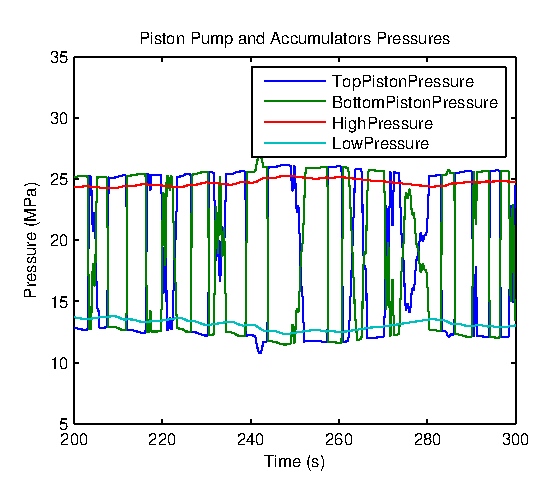
\includegraphics[width=1\columnwidth]{Images/Pressures}
    \caption{Piston Pump and Accumulators Pressures. A check valve is open when either the top or bottom piston pressure is greater than the high pressure accumulator or less than the low pressure accumulator.}
    %\label{fig-freq-comparison}
    \end{figure}

Fig. 10 shows the absorbed hydrodynamic power, the hydraulic system power, and the electrical generator output power.  The generator is modeled as a simple rotational inertia with a speed, torque, and efficiency lookup table based off of a typical large industrial induction generator. The average absorbed, mechanical, and electrical power are 110 kW, 81 kW, and 66 kW, respectively. The efficiency from absorbed to electrical power is 60~\%, while the efficiency from mechanical to electrical power is 82\%. 


%The motor efficiency was taken from ABB datasheet part number M3BJ315SMC.

\begin{figure}[t]
    \centering
    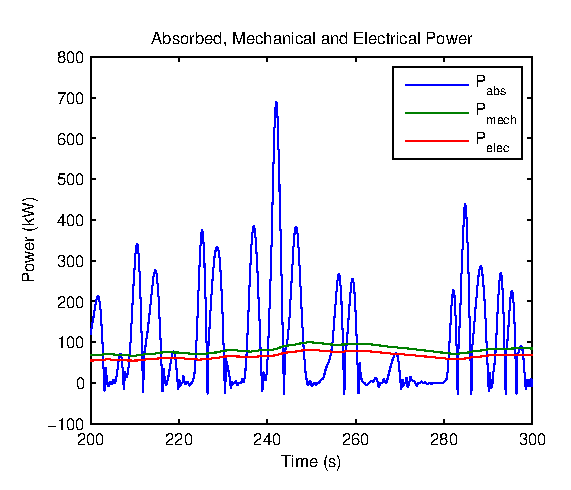
\includegraphics[width=1\columnwidth]{Images/Power}
    \caption{Absorbed, mechanical, and electrical power. The average absorbed power is 110 kW, the average mechanical power is 81 kW, and the average electrical power is 66 kW.}
    %\label{fig-freq-comparison}
    \end{figure}

\section{Conclusion}
WEC-Sim Version 1.0 which, released in summer 2014, has a power take off which is modeled as a simple linear damper. This paper presents the development and simulation of a WEC-Sim add-on package PTO-Sim, which enables the development of more complex PTO systems, including the hydraulic system that served as the example application of PTO-Sim in this paper. More PTO components will be developed for WEC-Sim, thus enabling WEC developers to quickly simulate many standard and custom PTO arrangements.

\section{Acknowledgments}
This research was made possible by support from the Wind and Water Power Technologies Office within the DOE Office of Energy Efficiency \& Renewable Energy. The work was supported by Sandia National Laboratories, a multi-program laboratory managed and operated by Sandia Corporation, a wholly owned subsidiary of Lockheed Martin Corporation, for the U.S. Department of Energy's National Nuclear Security Administration under contract DE-AC04-94AL85000.  Special thanks to Kelley Ruehl and Carlos Michelen for their support on the development of PTO-Sim.


% \section{Future Work}
% An actively controlled hydraulic PTO and direct-drive PTO will be modeled next. The actively controlled hydraulic drivetrain is a hydraulic PTO topology tracking an optimal power absorption trajectory.  A linear quadratic tracking controller will be developed to follow the reference trajectory. On the other hand, another candidate is the direct-drive power take-off, because it considered as a viable alternative to a hydraulic power take-off. This is mainly because of its simplistic design and higher efficiency.  
  



%\section{References}
%
%[1]	"WEC-Sim $|$ Open Energy Information." [Online]. Available: http://en.openei.org/wiki/WEC-Sim. [Accessed: 06-Nov-2014].\\
%
%[2]	Kelley Ruehl, Carlos Michelen, Samuel Kanner, Michael Lawson, and Y. Yu, "Preliminary
%Verification and Validation of WEC-Sim, an Open-Source Wave Energy Converter Design Tool," in Proceedings of OMAE 2014, San Francisco, CA, 2014.\\
%
%[3]	Y. Yu, Michael Lawson, Kelley Ruehl, and Carlos Michelen, "Development and Demonstration of the WEC-Sim Wave Energy Converter Simulation Tool," in Proceedings of the 2nd Marine Energy Technology Symposium, Seattle, WA, USA, 2014.\\
%
%[4]	Y. Yu, Ye Li, Kathleen Hallett, and Chad Hotimsky, "Design and Analysis for a Floating Oscillating Surge Wave Energy Converter," in Proceedings of OMAE 2014, San Francisco, CA, 2014.\\
%
%[5]	MJ Lawson, Y. Yu, Adam Nelessen, Kelley Ruehl, and Carlos Michelen, "Implementing Nonlinear Buoyancy and Excitation Forces in the WEC-Sim Wave Energy Converter Modeling Tool," in Proceedings of OMAE 2014, San Francisco, CA, 2014.\\
%
%[6]	"Sandia National Laboratories: Reference Model Project (RMP)." [Online]. Available:
%http://energy.sandia.gov/energy/renewable-energy/water-power/reference-model-projectrmp/$\#$.VFunP2PWODA. [Accessed: 06-Nov-2014].\\
%
%[7]	Michael C. Reed et al. "Accelerating U.S. Marine and Hydrokinetic Technology Development Through the Application of Technology Readiness Levels (TRLs)". In" Procedings of Energy Ocean International 2010, Ft. Lauderdale, FL (2010).\\
%
%[8]	K. Ruehl and D. Bull. "Wave Energy Development Roadmap: Design to commercialization". In: Oceans, 2012. 2012, pp. 1-10. DOI: 10.1109/OCEANS.2012.6404795.\\
%
%[9]	Det Norske Verita AS. "Recommended Practice DNV-RP-A203 Qualification Procedures for New Technology". In: Hvik. Norway (2001).\\
%
%[10] WHTP Marine Hydrokinetic Technologies Database: Project Profile. URL: http://www1.eere.energy.gov/water/hydrokinetic/ (visited on 07/01/2013).\\
%
%[11] Sean Casey, "Modeling, Simulation, and Analysis of Two Hydraulic Power Take-off Systems for Wave Energy Conversion," in ScholarsArchive@OSU 2013, Corvallis, OR, 2014.\\
%
%[12] Herbert E. Merritt. Hydraulic Control Systems. John Wiley $\&$ Sons, Inc., 1967.\\
%
%[13] Johannes Falnes. Ocean Waves and Oscillating Systems. Cambridge University Press, 2005.





%\cite{6225717}
\bibliographystyle{IEEEtran}  
\bibliography{ptosimbib}

\end{document}
